\documentclass[12pt,a4paper]{article}

\usepackage{buaa_paper}

\schoolname{北京航空航天大学计算机学院}
\title{硕士学位论文文献综述}
\papertitle{神经网络语言模型的性能优化研究}
\specialty{计算机科学与技术}
\studentnumber{SY1506330}
\researcharea{自然语言处理}
\advisor{荣文戈~~副教授}
\author{姜~~楠}
\date{2016 年 12 月 20 号}

\begin{document}

\maketitle



\addcontentsline{toc}{section}{摘要}
\keywords{神经语言模型;循环神经网络;层次多元概率模型}
{Neural Language Model;\ Recurrent Neural Network;\ Hierarchical Softmax}

\begin{abstract_ch}
  火焰动画的仿真和渲染作为流体计算力学在计算机图形学的一个重要应用之
  一,一直是一个很有挑战性的研究课题。近年来随着计算机硬件能力的提升
  和GPU并行计算的快速发展,具有高度真实感的实时火焰的模拟已经成为了研究
  的一个热点。

  本文首先介绍了火焰模拟的主要步骤,回顾了计算机图形学领域中对火焰的建模、绘制方法,以及
  火焰和环境交互下的主要模拟方法和算法。在建模方法中着重介绍了基于物理的火焰建模方法,即基于计算流体力学的模拟方法。然后重点讨论了火焰和环境交互时的相关研究成果。最后本文还展望了对于流体动画模
  拟未来发展的几个方向。
\end{abstract_ch}
\newpage
\begin{abstract_en}
  As one of the most important applications of Computational Fliud
  Dynamics in computer graphics, simulation of fire animation has been
  a chanllenging research topic. With the improvment of the computer
  hardware and rapid development of GPU parallel computing, simulation
  of highly realastic flame has become a research hotspot.


 Firstly, the main steps of flame simulation were presented, then we
will review the modeling and drawing methods of flame in the field of
computer graphics as well as the main simulation methods and
algorithms under the interaction of fire and environment. In the
modeling approach, we will focus on physics-based fire modeling, which
is the simulation methods based on computational fluid dynamics.
Afterwards, we will put emphasis to the relevant research results
about flame and environment interaction. Finally, this paper looked
ahead to the future development of the fluid animation in several
directions.

\end{abstract_en}
\newpage
\tableofcontents
\newpage

\section{引言}

近年来,随着Web2.0 的兴起,互联网上的数据急剧膨胀。根据国际数据公司(International Data Corp.,IDC)的统计和预测,2011 年全球网络数据量已经达到1.8ZB($1.8\times 10^6$TB),到2020 年,全球数据总量预计还将增长50 倍。大量无标注数据的出现,也让研究人员开始考虑,如何利用算法从这些大规模无标注的文本数据中自动挖掘规律,得到有用的信息。2006年, Hinton 提出的深度学习(Deep Learning, DL)\cite{hinton2006reducing}, 为解决这一问题带来了新的思路。在之后的发展中,基于神经网络的表示学习技术开始在各个领域崭露头角。尤其在图像和语音领域的多个任务上,基于表示学习的方法在性能上均超过了传统方法。

近年来,深度学习逐渐在自然语言处理中(Natural Language Processing, NLP)得到应用. 研究者提出用神经网络(Neural Network, NN) 来训练语言模型并进行了相关探索\cite{DBLP:conf/nips/BengioDV00}. 历史上,主要的语言建模方案(Language Modeling, LM)主要分为: 前馈神经网络语言模型和循环神经网络语言模型。其中,基于循环神经网络的语言模型建模方法引起了研究者极大的兴趣[3]. 网络通过学习能够将当前词的历史信息存储起来,以词的整个上下文(Context)作为依据,来预测下一个词出现的概率,克服了n-gram 语言模型无法利用语句中长距离上下文信息的缺点. 另外,在模型训练的过程中,由于词的历史信息被映射到低维连续空间,语义相似的词被聚类,在语料中出现次数较少的词仍然能够得到很好的训练,不再需要额外的数据平滑技术(Smoothing). 迄今为止,采用(Recurrent Neural Network, RNN)训练的语言模型在模型困惑度(Perplexity, PPL)和识别系统的识别率上都取得了最好的效果[4].

RNN 建模方法虽然表现出极大的优越性,却以牺牲计算复杂度为代价. 若训练大规模的文本语料,则需要花费很长的时间,制约了RNN 语言模型训练效率. 为克服这一不足,文献[5] 提出了多种优化策略来降低网络的计算复杂度,如缩短模型训练周期、减少训练数据集的规模、降低训练词典的大小、减少隐含层的节点数等,这些方法都在一定程度上降低了网络的运算量,提高了模型的训练效率,但同时也牺牲了较多的模型性能和冗余度. 另外,在网络结构层面上,文献\cite{DBLP:journals/coling/BrownPdLM92} 研究了一种基于分类的循环神经网络(Class-based RNN) 结构,网络的输出层被分解为两部分,增加的一部分称为分类层,从结构上降低了整个网络的计算复杂度,使得模型训练效率有了一定的提升且模型性能没有大的变化. 然而,在大词汇量连续语音识别系统中,采用此结构训练大规模语料语言模型仍需要花费大量时间. 因此,模型训练效率有待进一步优化.

因此探讨研究语言模型的大词表问题,是目前理论应用到实际过程中必须要克服的问题。我们当然可以通过配置高性能服务器来暂时延缓该问题的后果,但是一旦应用到大数据集上,即使是目前最好的中央处理单元(Central Processing Units, CPUs)或者图像处理单元(Graphical Processing Unit,GPU),仍然需要三五天时间才能训练完善。因此,在保证原有模型的准确率的目的下,如何提高模型的训练速度是我们主要讨论的内容。为此我们讨论了三个不同的方向:一种是通过采样技术(Importance Sampling)来减少必要的训练时间;一种是通过基于分类的多元分类(Class-based Hierarchical Softmax, cHSM)来加速模型; 最后一种是采用基于树模型的多层二元分类模型(Tree-based Hierarchical Softmax, tHSM). 同时,我们还需要针对CPU 和GPU设备分别进行探讨。因为传统的线性运算模型在流行的GPU并行运算方案中并不适用,需要结合不同的运算设备分别讨论可行的方案。

\section{国内外研究现状及发展动态}
\subsection{语言模型简介}
语言模型可以对一段文本的概率进行估计,对信息检索\cite{Jin:2002:TLM:564376.564386}、机器翻译\cite{DBLP:conf/naacl/BaltescuB15}、语音识别等任务有着重要的作用。
形式化讲,统计语言模型的作用是为一个长度为m 的字符串确定一个概率分布$P(w_1;w_2;\cdots;w_m)$,表示其存在的可能性,其中$w_1$ 到$w_m$ 依次表示这段文
本中的各个词。一般在实际求解过程中,通常采用下式计算其概率值:
\begin{equation}
\label{equ:lm}
\begin{split}
P(w_1;w_2; \cdots;w_m) &= P(w_1) P(w_2|w_1) P(w_3|w_1;w_2)\cdots P(w_i | w_1;w_2;\cdots;w_{i-1}) \\
&\cdots P(w_m | w_1;w_2;\cdots;w_{m-1})
\end{split}
\end{equation}
在实践中,如果文本的长度较长,公式\ref{equ:lm}右部$\cdots P(w_m | w_1;w_2;\cdots;w_{m-1}) $ 的估算会非常困难。因此,研究者们提出使用一个简化模型:n 元模型(n-gram model)。在n 元模型中估算条件概率时,距离大于等于n 的上文词会被忽略,也就是对上述条件概率做了以下近似:
\begin{equation}
\label{equ:approx}
P(w_i | w_1;w_2;\cdots;w_{i-1})  \approx P(w_i | w_{i-(n-1)};\cdots;w_{i-1})
\end{equation}
当$n = 1$ 时又称一元模型(unigram model),公式\ref{equ:approx} 右部会退化成$P(w_i)$,此时,整个句子的概率为:$P(w_1;w_2; \cdots;wm) = P(w_1)P(w_2) \cdots P(w_m)$。从式中可以知道,一元语言模型中,文本的概率为其中各词概率的乘积。也就是说,模型假设了各个词之间都是相互独立的,文本中的词序信息完全丢失。因此,该模型虽然估算方便,但性能有限。

当n = 2 时又称二元模型(bigram model),将n 代入公式\ref{equ:approx} 中,右部为P$(w_i|w_{i-1})$。常用的还有n = 3 时的三元模型(trigram model),使用$P(w_i |w_{i-2};w_{i-1})$ 作为近似。这些方法均可以保留一定的词序信息。



\section{语言模型概述}
\subsection{循环神经网络语言模型}
Mikolov等人提出的循环神经网络语言模型(Recurrent Neural Network based Language Model,RNNLM)则直接对$P(w_i | w_1;w_2;\cdots;w_{i-1}) $ 进行建模,而不使用公式\ref{equ:approx}对其进行简化\cite{mikolov2012statistical,DBLP:conf/interspeech/MikolovKBCK10}。因此,RNNLM 可以利用所有的上文信息,预测下一个词,其模型结构如图\ref{fig:rnnlm} 所示。
\begin{figure}
  \centering
  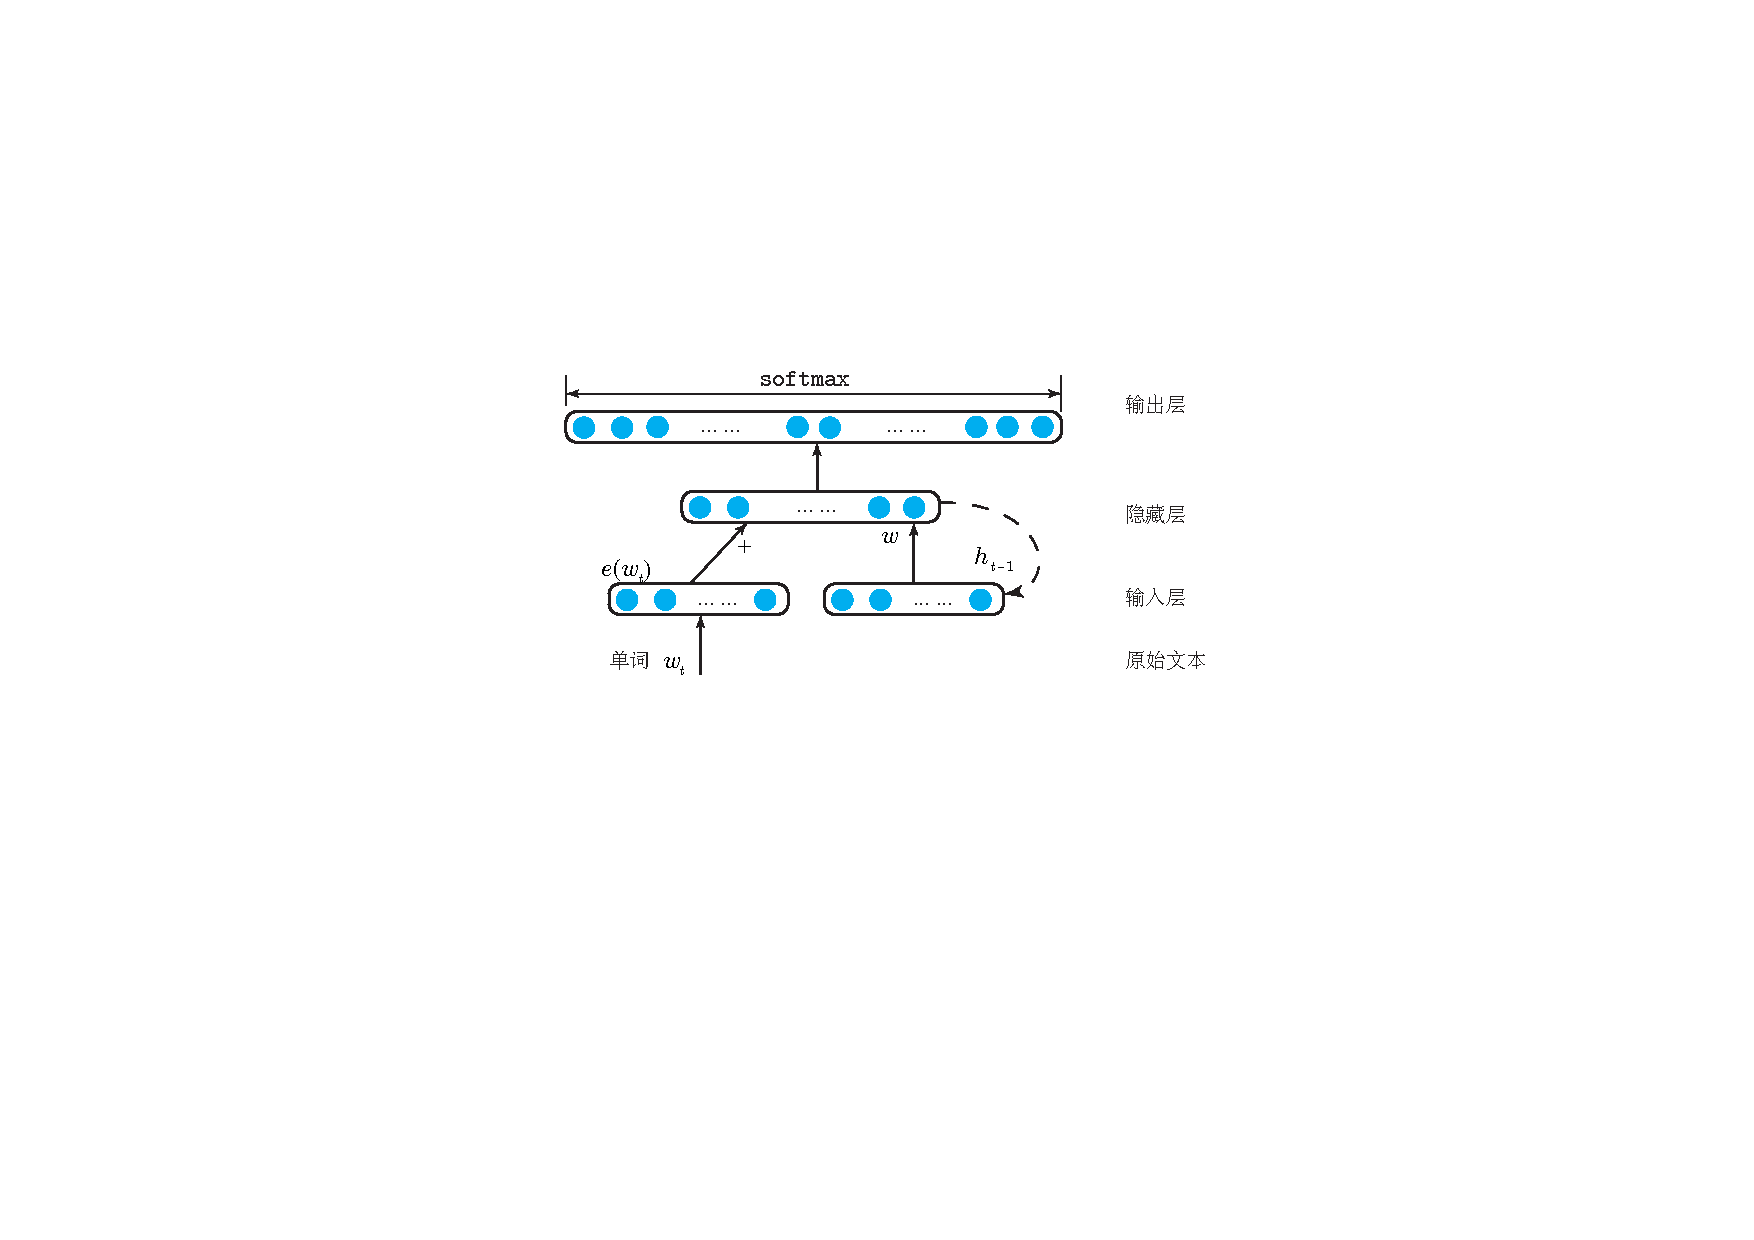
\includegraphics[width=0.85\linewidth]{./figures/rnnlm.png}
  \caption{循环神经网络语言模型(RNNLM)模型结构图}\label{fig:rnnlm}
\end{figure}




\subsection{对上下文信息建模策略}
依照上章节的分析,本章节主要介绍我们实验中所要涉及的模型,主要分为: 长短记忆网络(Long shrot-term memory, LSTM)和门限记忆节点(Gated Recurrent Unit,GRU)。

LSTM的计算公式定于如下:
\begin{itemize}
\item 输入门:控制输入的信息流:
$$i_t=\sigma(W^i x_t+U^i h_{t-1}+b^i)$$
\item  遗忘门:控制信息遗忘的速度:
$$f_t=\sigma(W^f x_t+U^f h_{t-1}+b^f)$$
\item  信息更新值:
$$g_t=\phi(W^g x_t+U^g h_{t-1}+b^g)$$
\item  输出门:
$$o_t=\sigma(W_o x_t+U^o h^{t-1}+b^o)$$
\item  中间状态更新:
$$s_t=g_t\cdot i_t+s_{t-1}\cdot f_t$$
\item  隐藏层的输出值:
$$h_t=s_t\cdot \phi(o_t)$$
\end{itemize}
其中$\cdot$ 代表"element-wise matrix multiplication"(对应元素相乘),$\phi(x)=\tanh(x),\sigma(x)=sigmoid(x)$
$$\phi(x)=\frac{e^x-e^{-x}}{e^x+e^{-x}},\sigma(x)=\frac{1}{1+e^{-x}}$$

GRU和lstm的计算公式很相似,具体定义如下:
\begin{itemize}
\item 更新门$z_t$: 定义保存多少以前的信息。

\[z_t = \sigma ( W^z x_t+ U^z h_{t-1}  )\]

\item 重置门$r_t$: 决定保留多少输入信息.

\[r_t = \sigma(W^r x_t  + U^r h_{t-1}  )\]

\item 节点内部更新值$\tilde h_t $:
 \[\tilde h_t  = \tanh (W^h x_t  + U^h(h_{t-1} \odot r_t) )\]

\item 隐藏层输出值$h_t$:
\[h_t = (1-z_t)\odot \tilde h_t  + z_t \odot h_{t-1}\]
\end{itemize}

\subsection{对多元分类模型的建模}
大词表问题,主要是对softmax如何建模的问题。在本课题中,我们探讨cHSM和tHSM两种不同的方案所带来的影响和优劣。
\subsection{单词聚类的策略}
当我们使用多层分类模型的时候,我们就需要将单词按照模型的架构进行划分。其中对于cHSM模型,我们有以下策略可以使用:1) 基于词频划分类别 2) 基于2-gram 的布朗聚类(brown clustering) 进行划分.3)按照word-embedding 的词向量信息进行聚类。另外,我们还需要注意的是,各个类别可以包含不同的数量的单词,也可以包含数量相同的单词。对于后者,我们考虑的划分模型就是基于交换算法(Exchange Algorithm), 以此来保证获得近似的最优解。



\section{总结与展望}
1) 数学背景和理论背景。 尽管本实验题目定义范围比较小,但是我们也需要很好的数学理论知识,包括:矩阵论,概率论。还有,我们还需要极强的阅读外文文献知识和编码实现能力,都是不可或缺的基本要求。

2) 基于theano框架的建模方案。因为基于 python 的深度学习库比较完善,适合建模。 本实验拟采用 theano 的建模语言,来帮助我们快速建模和调参。

3) 同时本实验也需要对linux的bash脚本有一定的熟悉,以方便将模型的数据结果正确的统计和运行模型的开发环境配置。

4) 试验结果图表统计和绘制.本实验的结果需要精良的语言来控制,而R语言的ggplot2框架就很适合我们的试验结果图表的绘制工作。

5) 基于GPU的cuda的模型优化也是我们需要考虑的问题之一。
\newpage
\addcontentsline{toc}{section}{主要参考文献}
\bibliography{bibs}

\end{document}
